
% Default to the notebook output style

    


% Inherit from the specified cell style.




    
\documentclass[12pt]{article}

    
    
    \usepackage[T1]{fontenc}
    % Nicer default font (+ math font) than Computer Modern for most use cases
    %\usepackage{mathpazo}

    % Basic figure setup, for now with no caption control since it's done
    % automatically by Pandoc (which extracts ![](path) syntax from Markdown).
    \usepackage{graphicx}
    % We will generate all images so they have a width \maxwidth. This means
    % that they will get their normal width if they fit onto the page, but
    % are scaled down if they would overflow the margins.
    %\makeatletter
    %\def\maxwidth{\ifdim\Gin@nat@width>\linewidth\linewidth
    %\else\Gin@nat@width\fi}
    %\makeatother
    %\let\Oldincludegraphics\includegraphics
    % Set max figure width to be 80% of text width, for now hardcoded.
    %\renewcommand{\includegraphics}[1]{\Oldincludegraphics[width=.8\maxwidth]{#1}}
    % Ensure that by default, figures have no caption (until we provide a
    % proper Figure object with a Caption API and a way to capture that
    % in the conversion process - todo).
    %\usepackage{caption}
    %\DeclareCaptionLabelFormat{nolabel}{}
    %\captionsetup{labelformat=nolabel}

    \usepackage{adjustbox} % Used to constrain images to a maximum size 
    \usepackage{xcolor} % Allow colors to be defined
    \usepackage{enumerate} % Needed for markdown enumerations to work
    \usepackage{geometry} % Used to adjust the document margins
    \usepackage{amsmath} % Equations
    \usepackage{amssymb} % Equations
    \usepackage{textcomp} % defines textquotesingle
    % Hack from http://tex.stackexchange.com/a/47451/13684:
    \AtBeginDocument{%
        \def\PYZsq{\textquotesingle}% Upright quotes in Pygmentized code
    }
    \usepackage{upquote} % Upright quotes for verbatim code
    \usepackage{eurosym} % defines \euro
    \usepackage[mathletters]{ucs} % Extended unicode (utf-8) support
    \usepackage[utf8x]{inputenc} % Allow utf-8 characters in the tex document
    \usepackage{fancyvrb} % verbatim replacement that allows latex
    \usepackage{grffile} % extends the file name processing of package graphics 
                         % to support a larger range 
    % The hyperref package gives us a pdf with properly built
    % internal navigation ('pdf bookmarks' for the table of contents,
    % internal cross-reference links, web links for URLs, etc.)
    \usepackage{hyperref}
    \usepackage{longtable} % longtable support required by pandoc >1.10
    \usepackage{booktabs}  % table support for pandoc > 1.12.2
    \usepackage[inline]{enumitem} % IRkernel/repr support (it uses the enumerate* environment)
    \usepackage[normalem]{ulem} % ulem is needed to support strikethroughs (\sout)
                                % normalem makes italics be italics, not underlines
    

    
    
    % Colors for the hyperref package
    \definecolor{urlcolor}{rgb}{0,.145,.698}
    \definecolor{linkcolor}{rgb}{.71,0.21,0.01}
    \definecolor{citecolor}{rgb}{.12,.54,.11}

    % ANSI colors
    \definecolor{ansi-black}{HTML}{3E424D}
    \definecolor{ansi-black-intense}{HTML}{282C36}
    \definecolor{ansi-red}{HTML}{E75C58}
    \definecolor{ansi-red-intense}{HTML}{B22B31}
    \definecolor{ansi-green}{HTML}{00A250}
    \definecolor{ansi-green-intense}{HTML}{007427}
    \definecolor{ansi-yellow}{HTML}{DDB62B}
    \definecolor{ansi-yellow-intense}{HTML}{B27D12}
    \definecolor{ansi-blue}{HTML}{208FFB}
    \definecolor{ansi-blue-intense}{HTML}{0065CA}
    \definecolor{ansi-magenta}{HTML}{D160C4}
    \definecolor{ansi-magenta-intense}{HTML}{A03196}
    \definecolor{ansi-cyan}{HTML}{60C6C8}
    \definecolor{ansi-cyan-intense}{HTML}{258F8F}
    \definecolor{ansi-white}{HTML}{C5C1B4}
    \definecolor{ansi-white-intense}{HTML}{A1A6B2}

    % commands and environments needed by pandoc snippets
    % extracted from the output of `pandoc -s`
    \providecommand{\tightlist}{%
      \setlength{\itemsep}{0pt}\setlength{\parskip}{0pt}}
    \DefineVerbatimEnvironment{Highlighting}{Verbatim}{commandchars=\\\{\}}
    % Add ',fontsize=\small' for more characters per line
    \newenvironment{Shaded}{}{}
    \newcommand{\KeywordTok}[1]{\textcolor[rgb]{0.00,0.44,0.13}{\textbf{{#1}}}}
    \newcommand{\DataTypeTok}[1]{\textcolor[rgb]{0.56,0.13,0.00}{{#1}}}
    \newcommand{\DecValTok}[1]{\textcolor[rgb]{0.25,0.63,0.44}{{#1}}}
    \newcommand{\BaseNTok}[1]{\textcolor[rgb]{0.25,0.63,0.44}{{#1}}}
    \newcommand{\FloatTok}[1]{\textcolor[rgb]{0.25,0.63,0.44}{{#1}}}
    \newcommand{\CharTok}[1]{\textcolor[rgb]{0.25,0.44,0.63}{{#1}}}
    \newcommand{\StringTok}[1]{\textcolor[rgb]{0.25,0.44,0.63}{{#1}}}
    \newcommand{\CommentTok}[1]{\textcolor[rgb]{0.38,0.63,0.69}{\textit{{#1}}}}
    \newcommand{\OtherTok}[1]{\textcolor[rgb]{0.00,0.44,0.13}{{#1}}}
    \newcommand{\AlertTok}[1]{\textcolor[rgb]{1.00,0.00,0.00}{\textbf{{#1}}}}
    \newcommand{\FunctionTok}[1]{\textcolor[rgb]{0.02,0.16,0.49}{{#1}}}
    \newcommand{\RegionMarkerTok}[1]{{#1}}
    \newcommand{\ErrorTok}[1]{\textcolor[rgb]{1.00,0.00,0.00}{\textbf{{#1}}}}
    \newcommand{\NormalTok}[1]{{#1}}
    
    % Additional commands for more recent versions of Pandoc
    \newcommand{\ConstantTok}[1]{\textcolor[rgb]{0.53,0.00,0.00}{{#1}}}
    \newcommand{\SpecialCharTok}[1]{\textcolor[rgb]{0.25,0.44,0.63}{{#1}}}
    \newcommand{\VerbatimStringTok}[1]{\textcolor[rgb]{0.25,0.44,0.63}{{#1}}}
    \newcommand{\SpecialStringTok}[1]{\textcolor[rgb]{0.73,0.40,0.53}{{#1}}}
    \newcommand{\ImportTok}[1]{{#1}}
    \newcommand{\DocumentationTok}[1]{\textcolor[rgb]{0.73,0.13,0.13}{\textit{{#1}}}}
    \newcommand{\AnnotationTok}[1]{\textcolor[rgb]{0.38,0.63,0.69}{\textbf{\textit{{#1}}}}}
    \newcommand{\CommentVarTok}[1]{\textcolor[rgb]{0.38,0.63,0.69}{\textbf{\textit{{#1}}}}}
    \newcommand{\VariableTok}[1]{\textcolor[rgb]{0.10,0.09,0.49}{{#1}}}
    \newcommand{\ControlFlowTok}[1]{\textcolor[rgb]{0.00,0.44,0.13}{\textbf{{#1}}}}
    \newcommand{\OperatorTok}[1]{\textcolor[rgb]{0.40,0.40,0.40}{{#1}}}
    \newcommand{\BuiltInTok}[1]{{#1}}
    \newcommand{\ExtensionTok}[1]{{#1}}
    \newcommand{\PreprocessorTok}[1]{\textcolor[rgb]{0.74,0.48,0.00}{{#1}}}
    \newcommand{\AttributeTok}[1]{\textcolor[rgb]{0.49,0.56,0.16}{{#1}}}
    \newcommand{\InformationTok}[1]{\textcolor[rgb]{0.38,0.63,0.69}{\textbf{\textit{{#1}}}}}
    \newcommand{\WarningTok}[1]{\textcolor[rgb]{0.38,0.63,0.69}{\textbf{\textit{{#1}}}}}
    
    
    % Define a nice break command that doesn't care if a line doesn't already
    % exist.
    \def\br{\hspace*{\fill} \\* }
    % Math Jax compatability definitions
    \def\gt{>}
    \def\lt{<}
    % Document parameters
    \title{Numerical Approximations of $\pi$}
    \author{Ian Mitchell\footnote{\url{Ian.Mitchell_001@gmx.com}}}
    \date{\today}
    
    

    % Pygments definitions
    
\makeatletter
\def\PY@reset{\let\PY@it=\relax \let\PY@bf=\relax%
    \let\PY@ul=\relax \let\PY@tc=\relax%
    \let\PY@bc=\relax \let\PY@ff=\relax}
\def\PY@tok#1{\csname PY@tok@#1\endcsname}
\def\PY@toks#1+{\ifx\relax#1\empty\else%
    \PY@tok{#1}\expandafter\PY@toks\fi}
\def\PY@do#1{\PY@bc{\PY@tc{\PY@ul{%
    \PY@it{\PY@bf{\PY@ff{#1}}}}}}}
\def\PY#1#2{\PY@reset\PY@toks#1+\relax+\PY@do{#2}}

\expandafter\def\csname PY@tok@w\endcsname{\def\PY@tc##1{\textcolor[rgb]{0.73,0.73,0.73}{##1}}}
\expandafter\def\csname PY@tok@c\endcsname{\let\PY@it=\textit\def\PY@tc##1{\textcolor[rgb]{0.25,0.50,0.50}{##1}}}
\expandafter\def\csname PY@tok@cp\endcsname{\def\PY@tc##1{\textcolor[rgb]{0.74,0.48,0.00}{##1}}}
\expandafter\def\csname PY@tok@k\endcsname{\let\PY@bf=\textbf\def\PY@tc##1{\textcolor[rgb]{0.00,0.50,0.00}{##1}}}
\expandafter\def\csname PY@tok@kp\endcsname{\def\PY@tc##1{\textcolor[rgb]{0.00,0.50,0.00}{##1}}}
\expandafter\def\csname PY@tok@kt\endcsname{\def\PY@tc##1{\textcolor[rgb]{0.69,0.00,0.25}{##1}}}
\expandafter\def\csname PY@tok@o\endcsname{\def\PY@tc##1{\textcolor[rgb]{0.40,0.40,0.40}{##1}}}
\expandafter\def\csname PY@tok@ow\endcsname{\let\PY@bf=\textbf\def\PY@tc##1{\textcolor[rgb]{0.67,0.13,1.00}{##1}}}
\expandafter\def\csname PY@tok@nb\endcsname{\def\PY@tc##1{\textcolor[rgb]{0.00,0.50,0.00}{##1}}}
\expandafter\def\csname PY@tok@nf\endcsname{\def\PY@tc##1{\textcolor[rgb]{0.00,0.00,1.00}{##1}}}
\expandafter\def\csname PY@tok@nc\endcsname{\let\PY@bf=\textbf\def\PY@tc##1{\textcolor[rgb]{0.00,0.00,1.00}{##1}}}
\expandafter\def\csname PY@tok@nn\endcsname{\let\PY@bf=\textbf\def\PY@tc##1{\textcolor[rgb]{0.00,0.00,1.00}{##1}}}
\expandafter\def\csname PY@tok@ne\endcsname{\let\PY@bf=\textbf\def\PY@tc##1{\textcolor[rgb]{0.82,0.25,0.23}{##1}}}
\expandafter\def\csname PY@tok@nv\endcsname{\def\PY@tc##1{\textcolor[rgb]{0.10,0.09,0.49}{##1}}}
\expandafter\def\csname PY@tok@no\endcsname{\def\PY@tc##1{\textcolor[rgb]{0.53,0.00,0.00}{##1}}}
\expandafter\def\csname PY@tok@nl\endcsname{\def\PY@tc##1{\textcolor[rgb]{0.63,0.63,0.00}{##1}}}
\expandafter\def\csname PY@tok@ni\endcsname{\let\PY@bf=\textbf\def\PY@tc##1{\textcolor[rgb]{0.60,0.60,0.60}{##1}}}
\expandafter\def\csname PY@tok@na\endcsname{\def\PY@tc##1{\textcolor[rgb]{0.49,0.56,0.16}{##1}}}
\expandafter\def\csname PY@tok@nt\endcsname{\let\PY@bf=\textbf\def\PY@tc##1{\textcolor[rgb]{0.00,0.50,0.00}{##1}}}
\expandafter\def\csname PY@tok@nd\endcsname{\def\PY@tc##1{\textcolor[rgb]{0.67,0.13,1.00}{##1}}}
\expandafter\def\csname PY@tok@s\endcsname{\def\PY@tc##1{\textcolor[rgb]{0.73,0.13,0.13}{##1}}}
\expandafter\def\csname PY@tok@sd\endcsname{\let\PY@it=\textit\def\PY@tc##1{\textcolor[rgb]{0.73,0.13,0.13}{##1}}}
\expandafter\def\csname PY@tok@si\endcsname{\let\PY@bf=\textbf\def\PY@tc##1{\textcolor[rgb]{0.73,0.40,0.53}{##1}}}
\expandafter\def\csname PY@tok@se\endcsname{\let\PY@bf=\textbf\def\PY@tc##1{\textcolor[rgb]{0.73,0.40,0.13}{##1}}}
\expandafter\def\csname PY@tok@sr\endcsname{\def\PY@tc##1{\textcolor[rgb]{0.73,0.40,0.53}{##1}}}
\expandafter\def\csname PY@tok@ss\endcsname{\def\PY@tc##1{\textcolor[rgb]{0.10,0.09,0.49}{##1}}}
\expandafter\def\csname PY@tok@sx\endcsname{\def\PY@tc##1{\textcolor[rgb]{0.00,0.50,0.00}{##1}}}
\expandafter\def\csname PY@tok@m\endcsname{\def\PY@tc##1{\textcolor[rgb]{0.40,0.40,0.40}{##1}}}
\expandafter\def\csname PY@tok@gh\endcsname{\let\PY@bf=\textbf\def\PY@tc##1{\textcolor[rgb]{0.00,0.00,0.50}{##1}}}
\expandafter\def\csname PY@tok@gu\endcsname{\let\PY@bf=\textbf\def\PY@tc##1{\textcolor[rgb]{0.50,0.00,0.50}{##1}}}
\expandafter\def\csname PY@tok@gd\endcsname{\def\PY@tc##1{\textcolor[rgb]{0.63,0.00,0.00}{##1}}}
\expandafter\def\csname PY@tok@gi\endcsname{\def\PY@tc##1{\textcolor[rgb]{0.00,0.63,0.00}{##1}}}
\expandafter\def\csname PY@tok@gr\endcsname{\def\PY@tc##1{\textcolor[rgb]{1.00,0.00,0.00}{##1}}}
\expandafter\def\csname PY@tok@ge\endcsname{\let\PY@it=\textit}
\expandafter\def\csname PY@tok@gs\endcsname{\let\PY@bf=\textbf}
\expandafter\def\csname PY@tok@gp\endcsname{\let\PY@bf=\textbf\def\PY@tc##1{\textcolor[rgb]{0.00,0.00,0.50}{##1}}}
\expandafter\def\csname PY@tok@go\endcsname{\def\PY@tc##1{\textcolor[rgb]{0.53,0.53,0.53}{##1}}}
\expandafter\def\csname PY@tok@gt\endcsname{\def\PY@tc##1{\textcolor[rgb]{0.00,0.27,0.87}{##1}}}
\expandafter\def\csname PY@tok@err\endcsname{\def\PY@bc##1{\setlength{\fboxsep}{0pt}\fcolorbox[rgb]{1.00,0.00,0.00}{1,1,1}{\strut ##1}}}
\expandafter\def\csname PY@tok@kc\endcsname{\let\PY@bf=\textbf\def\PY@tc##1{\textcolor[rgb]{0.00,0.50,0.00}{##1}}}
\expandafter\def\csname PY@tok@kd\endcsname{\let\PY@bf=\textbf\def\PY@tc##1{\textcolor[rgb]{0.00,0.50,0.00}{##1}}}
\expandafter\def\csname PY@tok@kn\endcsname{\let\PY@bf=\textbf\def\PY@tc##1{\textcolor[rgb]{0.00,0.50,0.00}{##1}}}
\expandafter\def\csname PY@tok@kr\endcsname{\let\PY@bf=\textbf\def\PY@tc##1{\textcolor[rgb]{0.00,0.50,0.00}{##1}}}
\expandafter\def\csname PY@tok@bp\endcsname{\def\PY@tc##1{\textcolor[rgb]{0.00,0.50,0.00}{##1}}}
\expandafter\def\csname PY@tok@fm\endcsname{\def\PY@tc##1{\textcolor[rgb]{0.00,0.00,1.00}{##1}}}
\expandafter\def\csname PY@tok@vc\endcsname{\def\PY@tc##1{\textcolor[rgb]{0.10,0.09,0.49}{##1}}}
\expandafter\def\csname PY@tok@vg\endcsname{\def\PY@tc##1{\textcolor[rgb]{0.10,0.09,0.49}{##1}}}
\expandafter\def\csname PY@tok@vi\endcsname{\def\PY@tc##1{\textcolor[rgb]{0.10,0.09,0.49}{##1}}}
\expandafter\def\csname PY@tok@vm\endcsname{\def\PY@tc##1{\textcolor[rgb]{0.10,0.09,0.49}{##1}}}
\expandafter\def\csname PY@tok@sa\endcsname{\def\PY@tc##1{\textcolor[rgb]{0.73,0.13,0.13}{##1}}}
\expandafter\def\csname PY@tok@sb\endcsname{\def\PY@tc##1{\textcolor[rgb]{0.73,0.13,0.13}{##1}}}
\expandafter\def\csname PY@tok@sc\endcsname{\def\PY@tc##1{\textcolor[rgb]{0.73,0.13,0.13}{##1}}}
\expandafter\def\csname PY@tok@dl\endcsname{\def\PY@tc##1{\textcolor[rgb]{0.73,0.13,0.13}{##1}}}
\expandafter\def\csname PY@tok@s2\endcsname{\def\PY@tc##1{\textcolor[rgb]{0.73,0.13,0.13}{##1}}}
\expandafter\def\csname PY@tok@sh\endcsname{\def\PY@tc##1{\textcolor[rgb]{0.73,0.13,0.13}{##1}}}
\expandafter\def\csname PY@tok@s1\endcsname{\def\PY@tc##1{\textcolor[rgb]{0.73,0.13,0.13}{##1}}}
\expandafter\def\csname PY@tok@mb\endcsname{\def\PY@tc##1{\textcolor[rgb]{0.40,0.40,0.40}{##1}}}
\expandafter\def\csname PY@tok@mf\endcsname{\def\PY@tc##1{\textcolor[rgb]{0.40,0.40,0.40}{##1}}}
\expandafter\def\csname PY@tok@mh\endcsname{\def\PY@tc##1{\textcolor[rgb]{0.40,0.40,0.40}{##1}}}
\expandafter\def\csname PY@tok@mi\endcsname{\def\PY@tc##1{\textcolor[rgb]{0.40,0.40,0.40}{##1}}}
\expandafter\def\csname PY@tok@il\endcsname{\def\PY@tc##1{\textcolor[rgb]{0.40,0.40,0.40}{##1}}}
\expandafter\def\csname PY@tok@mo\endcsname{\def\PY@tc##1{\textcolor[rgb]{0.40,0.40,0.40}{##1}}}
\expandafter\def\csname PY@tok@ch\endcsname{\let\PY@it=\textit\def\PY@tc##1{\textcolor[rgb]{0.25,0.50,0.50}{##1}}}
\expandafter\def\csname PY@tok@cm\endcsname{\let\PY@it=\textit\def\PY@tc##1{\textcolor[rgb]{0.25,0.50,0.50}{##1}}}
\expandafter\def\csname PY@tok@cpf\endcsname{\let\PY@it=\textit\def\PY@tc##1{\textcolor[rgb]{0.25,0.50,0.50}{##1}}}
\expandafter\def\csname PY@tok@c1\endcsname{\let\PY@it=\textit\def\PY@tc##1{\textcolor[rgb]{0.25,0.50,0.50}{##1}}}
\expandafter\def\csname PY@tok@cs\endcsname{\let\PY@it=\textit\def\PY@tc##1{\textcolor[rgb]{0.25,0.50,0.50}{##1}}}

\def\PYZbs{\char`\\}
\def\PYZus{\char`\_}
\def\PYZob{\char`\{}
\def\PYZcb{\char`\}}
\def\PYZca{\char`\^}
\def\PYZam{\char`\&}
\def\PYZlt{\char`\<}
\def\PYZgt{\char`\>}
\def\PYZsh{\char`\#}
\def\PYZpc{\char`\%}
\def\PYZdl{\char`\$}
\def\PYZhy{\char`\-}
\def\PYZsq{\char`\'}
\def\PYZdq{\char`\"}
\def\PYZti{\char`\~}
% for compatibility with earlier versions
\def\PYZat{@}
\def\PYZlb{[}
\def\PYZrb{]}
\makeatother


    % Exact colors from NB
    \definecolor{incolor}{rgb}{0.0, 0.0, 0.5}
    \definecolor{outcolor}{rgb}{0.545, 0.0, 0.0}



    
    % Prevent overflowing lines due to hard-to-break entities
    \sloppy 
    % Setup hyperref package
    \hypersetup{
      breaklinks=true,  % so long urls are correctly broken across lines
      colorlinks=true,
      urlcolor=urlcolor,
      linkcolor=linkcolor,
      citecolor=citecolor,
      }
    % Slightly bigger margins than the latex defaults
    
    \geometry{verbose,tmargin=1in,bmargin=1in,lmargin=1in,rmargin=1in}
    
    

    \begin{document}
    
    
    \maketitle
    
    

    
%    \hypertarget{numerical-approximations-of-pi}{%
%\section{\texorpdfstring{NUMERICAL APPROXIMATIONS OF
%\(\pi\)}{NUMERICAL APPROXIMATIONS OF \textbackslash{}pi}}\label{numerical-approximations-of-pi}}

%\hypertarget{ian-mitchell-ian.mitchell_001gmx.com}{%
%\subsection{\texorpdfstring{Ian Mitchell,
%\href{mailto:Ian.Mitchell_001@gmx.com}{\nolinkurl{Ian.Mitchell\_001@gmx.com}}}{Ian Mitchell, Ian.Mitchell\_001@gmx.com}}\label{ian-mitchell-ian.mitchell_001gmx.com}}

\begin{abstract}
Python has allowed for \(\pi\) to be approximated in many easier ways than before. Using an algorithm where an \(n\) number of points are placed and the areas of a square and a circle are compared, \(\pi\) can be approximated to varying degrees of accuracy. However, the algorithm is a very brute-force method, and can heavily use system resources. In general, it would be easier to symbollicaly or numerically solve a Gaussian integral.
\end{abstract}


\section{Introduction and Trial}

\(\pi\) can be numerically approximated using many different methods. However, in this case, we are using a recursive Monte-carlo-like method in Python to essentially average all the areas of the circle. To compare, the Gaussian integral \(f(x) = \big(\int_{-\infty}^\infty e^{-x^2}\,dx\big)^2 = \pi\) is used. It can be noted that \(e\) is an irrational number itself. However, \(e\) has a few clear definitions such as \(e = \sum_{k = 0}^{\infty} \frac{1}{k!}\).

It can be noted that the accuracy in which the algorithm measures \(\pi\) at increases signifigantly increases with each decimal place. You can see based on the table of trials below. A total of 10 trials were done for each of the values of \(n\).

\begin{longtable}[]{@{}ccccc@{}}
\toprule
\(n = 10\) & \(n = 100\) & \(n = 1000\) & \(n = 10000\) &
\(n = 100000\)\tabularnewline
\midrule
\endhead
2.8 & 3.12 & 3.18 & 3.1104 & 3.147\tabularnewline
3.2 & 3.16 & 3.124 & 3.146 & 3.14876\tabularnewline
3.6 & 3.24 & 3.168 & 3.1332 & 3.15028\tabularnewline
3.6 & 2.8 & 3.164 & 3.1544 & 3.1456\tabularnewline
3.2 & 3.12 & 3.192 & 3.1496 & 3.1436\tabularnewline
1.6 & 3.08 & 3.056 & 3.0976 & 3.135\tabularnewline
2.4 & 3.08 & 3.132 & 3.1508 & 3.14416\tabularnewline
3.2 & 3.0 & 3.08 & 3.1352 & 3.14248\tabularnewline
2.8 & 3.44 & 3.048 & 3.1476 & 3.13816\tabularnewline
2.4 & 3.16 & 3.14 & 3.1372 & 3.14184\tabularnewline
\bottomrule
\caption{Values of $\pi$ put through the approximater.}
\end{longtable}

%\begin{center}
%\emph{Table 1: Values of \(\pi\) put through the approximater.}
%\end{center}

\begin{figure}[h]
\centering	
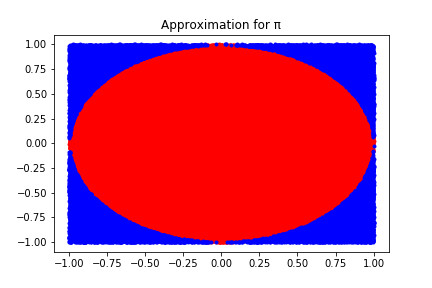
\includegraphics[scale=0.5]{pi_pictures/approx.jpg}
\caption{$\pi$ approximated to $n = 100000$ places.}
\end{figure}

\begin{figure}[h]
\centering
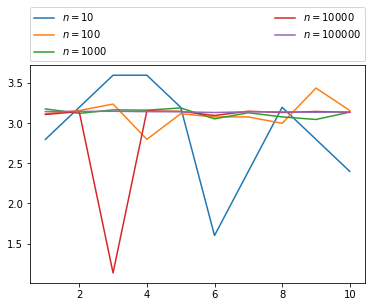
\includegraphics[scale=0.5]{pi_pictures/index.png} 
\caption{Values of the approximation for \(\pi\).}
\end{figure}

\begin{longtable}[]{@{}ccccc@{}}
\toprule
\(n = 10\) & \(n = 100\) & \(n = 1000\) & \(n = 10000\) &
\(n = 100000\)\tabularnewline
\midrule
\endhead
0.58788 & 0.15492 & 0.04874 & 0.60126 & 0.00442\tabularnewline
\bottomrule
\caption{Standard deviation for each value of $n$.}
\end{longtable}
[\footnote{$\sigma = \sum_i \sqrt{\frac{(x_i - \bar{x})^2}{n - 2}}$}]
\newpage

\section{Conclusions}
As can be seen from the graph, the graph allows for the circle to go outside of what a circle is. This can mess up the values of \(\pi\) since the area is different than that of a \emph{true} cirle's area. However, the actual size of the `circle' is rather similar to a true \emph{circle}. Yet, it is accurate provided enough points are given. The main fault of this can simply be tossed away if one were to use the Gaussian integral
\[f(x) = \bigg(\int_{-\infty}^\infty e^{-x^2}\,dx\bigg)^2 = \pi\,.\]
The use of this integral would serve to be much simpler on calculations and on computer resources. However, problems arise if one does not have a library or program for any sort of symbolic computation (i.e.~SymPy, Maxima, or Mathematica\texttrademark). Yet, the resources used by this algorithm is far more taxing on system resources---negating this solution for lower-performing computers.

\section{Code}

    \begin{Verbatim}[commandchars=\\\{\}]
{\color{incolor}In [{\color{incolor}1}]:} \PY{c+c1}{\PYZsh{}\PYZsh{}\PYZsh{} PI APPROXIMATER \PYZsh{}\PYZsh{}\PYZsh{} }
        \PY{o}{\PYZpc{}}\PY{k}{matplotlib} inline
        
        \PY{k+kn}{import} \PY{n+nn}{matplotlib}\PY{n+nn}{.}\PY{n+nn}{pyplot} \PY{k}{as} \PY{n+nn}{plt}
        \PY{k+kn}{import} \PY{n+nn}{numpy} \PY{k}{as} \PY{n+nn}{np}
        \PY{k+kn}{from} \PY{n+nn}{numpy} \PY{k}{import} \PY{n}{random}
        \PY{k+kn}{from} \PY{n+nn}{sympy} \PY{k}{import} \PY{o}{*}
        
        \PY{c+c1}{\PYZsh{} Sympy approximation}
        
        \PY{n}{X} \PY{o}{=} \PY{n}{symbols}\PY{p}{(}\PY{l+s+s1}{\PYZsq{}}\PY{l+s+s1}{X}\PY{l+s+s1}{\PYZsq{}}\PY{p}{)}
        
        \PY{n}{f} \PY{o}{=} \PY{n}{exp}\PY{p}{(}\PY{o}{\PYZhy{}}\PY{p}{(}\PY{n}{X}\PY{o}{*}\PY{o}{*}\PY{l+m+mi}{2}\PY{p}{)}\PY{p}{)}
        
        \PY{n}{Pi\PYZus{}1} \PY{o}{=} \PY{n}{N}\PY{p}{(}\PY{p}{(}\PY{n}{integrate}\PY{p}{(}\PY{n}{f}\PY{p}{,} \PY{p}{(}\PY{n}{X}\PY{p}{,} \PY{o}{\PYZhy{}}\PY{n}{oo}\PY{p}{,} \PY{n}{oo}\PY{p}{)}\PY{p}{)}\PY{p}{)}\PY{o}{*}\PY{o}{*}\PY{l+m+mi}{2}\PY{p}{)}
        
        \PY{c+c1}{\PYZsh{} \PYZhy{}\PYZhy{}\PYZhy{}\PYZhy{}}
        
        \PY{c+c1}{\PYZsh{} Numpy approximation}
        \PY{c+c1}{\PYZsh{}\PYZsh{} Credit to Andrew Dotson with his video \PYZdq{}How to Estimate Pi Numerically in Python\PYZdq{}. \PYZlt{}https://www.youtube.com/watch?v=JjfrNc\PYZhy{}G\PYZhy{}zA\PYZgt{}}
        
        \PY{n}{n} \PY{o}{=} \PY{n+nb}{input}\PY{p}{(}\PY{l+s+s2}{\PYZdq{}}\PY{l+s+s2}{Input the number of points. n = }\PY{l+s+s2}{\PYZdq{}}\PY{p}{)} \PY{c+c1}{\PYZsh{} Number of points}
        \PY{c+c1}{\PYZsh{} print(\PYZsq{}Input your amount of points. n = \PYZsq{})}
        
        \PY{n}{circlex} \PY{o}{=} \PY{p}{[}\PY{p}{]}
        \PY{n}{circley} \PY{o}{=} \PY{p}{[}\PY{p}{]}
        
        \PY{n}{squarex} \PY{o}{=} \PY{p}{[}\PY{p}{]}
        \PY{n}{squarey} \PY{o}{=} \PY{p}{[}\PY{p}{]}
        
        \PY{n}{i} \PY{o}{=} \PY{l+m+mi}{1}
        
        \PY{c+c1}{\PYZsh{} Approximation for pi}
        \PY{k}{while} \PY{n}{i}\PY{o}{\PYZlt{}}\PY{o}{=}\PY{n+nb}{int}\PY{p}{(}\PY{n}{n}\PY{p}{)}\PY{p}{:}
            \PY{n}{x} \PY{o}{=} \PY{n}{random}\PY{o}{.}\PY{n}{uniform}\PY{p}{(}\PY{o}{\PYZhy{}}\PY{l+m+mi}{1}\PY{p}{,} \PY{l+m+mi}{1}\PY{p}{)}
            \PY{n}{y} \PY{o}{=} \PY{n}{random}\PY{o}{.}\PY{n}{uniform}\PY{p}{(}\PY{o}{\PYZhy{}}\PY{l+m+mi}{1}\PY{p}{,} \PY{l+m+mi}{1}\PY{p}{)}
            \PY{k}{if} \PY{p}{(}\PY{n}{x}\PY{o}{*}\PY{o}{*}\PY{l+m+mi}{2} \PY{o}{+} \PY{n}{y}\PY{o}{*}\PY{o}{*}\PY{l+m+mi}{2} \PY{o}{\PYZlt{}}\PY{o}{=} \PY{l+m+mi}{1}\PY{p}{)}\PY{p}{:}
                \PY{n}{circlex}\PY{o}{.}\PY{n}{append}\PY{p}{(}\PY{n}{x}\PY{p}{)}
                \PY{n}{circley}\PY{o}{.}\PY{n}{append}\PY{p}{(}\PY{n}{y}\PY{p}{)}
            \PY{k}{else}\PY{p}{:} 
                \PY{n}{squarex}\PY{o}{.}\PY{n}{append}\PY{p}{(}\PY{n}{x}\PY{p}{)}
                \PY{n}{squarey}\PY{o}{.}\PY{n}{append}\PY{p}{(}\PY{n}{y}\PY{p}{)}
            \PY{n}{i}\PY{o}{+}\PY{o}{=}\PY{l+m+mi}{1}
        
            
        \PY{n}{Pi\PYZus{}2} \PY{o}{=} \PY{l+m+mi}{4}\PY{o}{*}\PY{n+nb}{len}\PY{p}{(}\PY{n}{circlex}\PY{p}{)}\PY{o}{/}\PY{n+nb}{float}\PY{p}{(}\PY{n}{n}\PY{p}{)}
        
        \PY{n}{plt}\PY{o}{.}\PY{n}{plot}\PY{p}{(}\PY{n}{circlex}\PY{p}{,}\PY{n}{circley}\PY{p}{,}\PY{l+s+s1}{\PYZsq{}}\PY{l+s+s1}{r.}\PY{l+s+s1}{\PYZsq{}}\PY{p}{)}
        \PY{n}{plt}\PY{o}{.}\PY{n}{plot}\PY{p}{(}\PY{n}{squarex}\PY{p}{,}\PY{n}{squarey}\PY{p}{,}\PY{l+s+s1}{\PYZsq{}}\PY{l+s+s1}{b.}\PY{l+s+s1}{\PYZsq{}}\PY{p}{)}
        \PY{n}{plt}\PY{o}{.}\PY{n}{grid}
        \PY{n}{plt}\PY{o}{.}\PY{n}{title}\PY{p}{(}\PY{l+s+s1}{\PYZsq{}}\PY{l+s+s1}{Approximation for π}\PY{l+s+s1}{\PYZsq{}}\PY{p}{)}
        \PY{c+c1}{\PYZsh{} Plot the approximation}
        
        \PY{c+c1}{\PYZsh{} \PYZhy{}\PYZhy{}\PYZhy{}\PYZhy{}}
        
        \PY{n+nb}{print}\PY{p}{(}\PY{l+s+s2}{\PYZdq{}}\PY{l+s+s2}{According to sympy, π is equal to }\PY{l+s+si}{\PYZob{}0\PYZcb{}}\PY{l+s+s2}{. However, the circle approximated it as }\PY{l+s+si}{\PYZob{}1\PYZcb{}}\PY{l+s+s2}{.}\PY{l+s+s2}{\PYZdq{}}\PY{o}{.}\PY{n}{format}\PY{p}{(}\PY{n}{Pi\PYZus{}1}\PY{p}{,} \PY{n}{Pi\PYZus{}2}\PY{p}{)}\PY{p}{)}
\end{Verbatim}


    \begin{Verbatim}[commandchars=\\\{\}]
According to sympy, π is equal to 3.14159265358979. However, the circle approximated it as 3.44.

    \end{Verbatim}

    \begin{center}
    \adjustimage{max size={0.9\linewidth}{0.9\paperheight}}{output_1_1.png}
    \end{center}
    { \hspace*{\fill} \\}
    
    \begin{Verbatim}[commandchars=\\\{\}]
{\color{incolor}In [{\color{incolor}2}]:} \PY{c+c1}{\PYZsh{}\PYZsh{}\PYZsh{} STANDARD DEVIATION OF THE POINTS FROM THE APPROXIMATER \PYZsh{}\PYZsh{}\PYZsh{} }
        
        \PY{k+kn}{import} \PY{n+nn}{matplotlib}\PY{n+nn}{.}\PY{n+nn}{pyplot} \PY{k}{as} \PY{n+nn}{plt}
        \PY{k+kn}{import} \PY{n+nn}{numpy} \PY{k}{as} \PY{n+nn}{np}
        \PY{k+kn}{from} \PY{n+nn}{numpy} \PY{k}{import} \PY{n}{random}
        \PY{k+kn}{from} \PY{n+nn}{sympy} \PY{k}{import} \PY{o}{*}
        
        \PY{n}{A} \PY{o}{=} \PY{p}{[}\PY{l+m+mf}{2.8}\PY{p}{,} \PY{l+m+mf}{3.2}\PY{p}{,} \PY{l+m+mf}{3.6}\PY{p}{,} \PY{l+m+mf}{3.6}\PY{p}{,} \PY{l+m+mf}{3.2}\PY{p}{,} \PY{l+m+mf}{1.6}\PY{p}{,} \PY{l+m+mf}{2.4}\PY{p}{,} \PY{l+m+mf}{3.2}\PY{p}{,} \PY{l+m+mf}{2.8}\PY{p}{,} \PY{l+m+mf}{2.4}\PY{p}{]}
        \PY{n}{B} \PY{o}{=} \PY{p}{[}\PY{l+m+mf}{3.12}\PY{p}{,} \PY{l+m+mf}{3.16}\PY{p}{,} \PY{l+m+mf}{3.24}\PY{p}{,} \PY{l+m+mf}{2.8}\PY{p}{,} \PY{l+m+mf}{3.12}\PY{p}{,} \PY{l+m+mf}{3.08}\PY{p}{,} \PY{l+m+mf}{3.08}\PY{p}{,} \PY{l+m+mf}{3.0}\PY{p}{,} \PY{l+m+mf}{3.44}\PY{p}{,} \PY{l+m+mf}{3.16}\PY{p}{]}
        \PY{n}{C} \PY{o}{=} \PY{p}{[}\PY{l+m+mf}{3.18}\PY{p}{,} \PY{l+m+mf}{3.124}\PY{p}{,} \PY{l+m+mf}{3.168}\PY{p}{,} \PY{l+m+mf}{3.164}\PY{p}{,} \PY{l+m+mf}{3.192}\PY{p}{,} \PY{l+m+mf}{3.056}\PY{p}{,} \PY{l+m+mf}{3.132}\PY{p}{,} \PY{l+m+mf}{3.08}\PY{p}{,} \PY{l+m+mf}{3.048}\PY{p}{,} \PY{l+m+mf}{3.14}\PY{p}{]}
        \PY{n}{D} \PY{o}{=} \PY{p}{[}\PY{l+m+mf}{3.1104}\PY{p}{,} \PY{l+m+mf}{3.146}\PY{p}{,} \PY{l+m+mf}{1.1332}\PY{p}{,} \PY{l+m+mf}{3.1544}\PY{p}{,} \PY{l+m+mf}{3.1496}\PY{p}{,} \PY{l+m+mf}{3.0976}\PY{p}{,} \PY{l+m+mf}{3.1508}\PY{p}{,} \PY{l+m+mf}{3.1352}\PY{p}{,} \PY{l+m+mf}{3.1476}\PY{p}{,} \PY{l+m+mf}{3.1372}\PY{p}{]}
        \PY{n}{E} \PY{o}{=} \PY{p}{[}\PY{l+m+mf}{3.147}\PY{p}{,} \PY{l+m+mf}{3.14876}\PY{p}{,} \PY{l+m+mf}{3.15028}\PY{p}{,} \PY{l+m+mf}{3.1456}\PY{p}{,} \PY{l+m+mf}{3.1436}\PY{p}{,} \PY{l+m+mf}{3.135}\PY{p}{,} \PY{l+m+mf}{3.14416}\PY{p}{,} \PY{l+m+mf}{3.14248}\PY{p}{,} \PY{l+m+mf}{3.13816}\PY{p}{,} \PY{l+m+mf}{3.14184}\PY{p}{]}
        
        \PY{n}{dev\PYZus{}A} \PY{o}{=} \PY{n}{np}\PY{o}{.}\PY{n}{round}\PY{p}{(}\PY{n}{np}\PY{o}{.}\PY{n}{std}\PY{p}{(}\PY{n}{A}\PY{p}{)}\PY{p}{,}\PY{l+m+mi}{5}\PY{p}{)}
        \PY{n}{dev\PYZus{}B} \PY{o}{=} \PY{n}{np}\PY{o}{.}\PY{n}{round}\PY{p}{(}\PY{n}{np}\PY{o}{.}\PY{n}{std}\PY{p}{(}\PY{n}{B}\PY{p}{)}\PY{p}{,}\PY{l+m+mi}{5}\PY{p}{)}
        \PY{n}{dev\PYZus{}C} \PY{o}{=} \PY{n}{np}\PY{o}{.}\PY{n}{round}\PY{p}{(}\PY{n}{np}\PY{o}{.}\PY{n}{std}\PY{p}{(}\PY{n}{C}\PY{p}{)}\PY{p}{,}\PY{l+m+mi}{5}\PY{p}{)}
        \PY{n}{dev\PYZus{}D} \PY{o}{=} \PY{n}{np}\PY{o}{.}\PY{n}{round}\PY{p}{(}\PY{n}{np}\PY{o}{.}\PY{n}{std}\PY{p}{(}\PY{n}{D}\PY{p}{)}\PY{p}{,}\PY{l+m+mi}{5}\PY{p}{)}
        \PY{n}{dev\PYZus{}E} \PY{o}{=} \PY{n}{np}\PY{o}{.}\PY{n}{round}\PY{p}{(}\PY{n}{np}\PY{o}{.}\PY{n}{std}\PY{p}{(}\PY{n}{E}\PY{p}{)}\PY{p}{,}\PY{l+m+mi}{5}\PY{p}{)}
        
        \PY{n+nb}{print}\PY{p}{(}\PY{l+s+s2}{\PYZdq{}}\PY{l+s+s2}{|}\PY{l+s+si}{\PYZob{}0\PYZcb{}}\PY{l+s+s2}{|}\PY{l+s+si}{\PYZob{}1\PYZcb{}}\PY{l+s+s2}{|}\PY{l+s+si}{\PYZob{}2\PYZcb{}}\PY{l+s+s2}{|}\PY{l+s+si}{\PYZob{}3\PYZcb{}}\PY{l+s+s2}{|}\PY{l+s+si}{\PYZob{}4\PYZcb{}}\PY{l+s+s2}{|}\PY{l+s+s2}{\PYZdq{}}\PY{o}{.}\PY{n}{format}\PY{p}{(}\PY{n}{dev\PYZus{}A}\PY{p}{,} \PY{n}{dev\PYZus{}B}\PY{p}{,} \PY{n}{dev\PYZus{}C}\PY{p}{,} \PY{n}{dev\PYZus{}D}\PY{p}{,} \PY{n}{dev\PYZus{}E}\PY{p}{)}\PY{p}{)}
\end{Verbatim}


    \begin{Verbatim}[commandchars=\\\{\}]
|0.58788|0.15492|0.04874|0.60126|0.00442|

    \end{Verbatim}

    \begin{Verbatim}[commandchars=\\\{\}]
{\color{incolor}In [{\color{incolor}3}]:} \PY{c+c1}{\PYZsh{}\PYZsh{}\PYZsh{} PLOT OF THE POINTS FOR THE APPROXIMATER \PYZsh{}\PYZsh{}\PYZsh{}}
        \PY{o}{\PYZpc{}}\PY{k}{matplotlib} inline
        
        \PY{k+kn}{import} \PY{n+nn}{matplotlib}\PY{n+nn}{.}\PY{n+nn}{pyplot} \PY{k}{as} \PY{n+nn}{plt}
        \PY{k+kn}{import} \PY{n+nn}{numpy} \PY{k}{as} \PY{n+nn}{np}
        \PY{k+kn}{from} \PY{n+nn}{numpy} \PY{k}{import} \PY{n}{random}
        \PY{k+kn}{from} \PY{n+nn}{sympy} \PY{k}{import} \PY{o}{*}
        
        \PY{n}{A} \PY{o}{=} \PY{p}{[}\PY{l+m+mf}{2.8}\PY{p}{,} \PY{l+m+mf}{3.2}\PY{p}{,} \PY{l+m+mf}{3.6}\PY{p}{,} \PY{l+m+mf}{3.6}\PY{p}{,} \PY{l+m+mf}{3.2}\PY{p}{,} \PY{l+m+mf}{1.6}\PY{p}{,} \PY{l+m+mf}{2.4}\PY{p}{,} \PY{l+m+mf}{3.2}\PY{p}{,} \PY{l+m+mf}{2.8}\PY{p}{,} \PY{l+m+mf}{2.4}\PY{p}{]}
        \PY{n}{B} \PY{o}{=} \PY{p}{[}\PY{l+m+mf}{3.12}\PY{p}{,} \PY{l+m+mf}{3.16}\PY{p}{,} \PY{l+m+mf}{3.24}\PY{p}{,} \PY{l+m+mf}{2.8}\PY{p}{,} \PY{l+m+mf}{3.12}\PY{p}{,} \PY{l+m+mf}{3.08}\PY{p}{,} \PY{l+m+mf}{3.08}\PY{p}{,} \PY{l+m+mf}{3.0}\PY{p}{,} \PY{l+m+mf}{3.44}\PY{p}{,} \PY{l+m+mf}{3.16}\PY{p}{]}
        \PY{n}{C} \PY{o}{=} \PY{p}{[}\PY{l+m+mf}{3.18}\PY{p}{,} \PY{l+m+mf}{3.124}\PY{p}{,} \PY{l+m+mf}{3.168}\PY{p}{,} \PY{l+m+mf}{3.164}\PY{p}{,} \PY{l+m+mf}{3.192}\PY{p}{,} \PY{l+m+mf}{3.056}\PY{p}{,} \PY{l+m+mf}{3.132}\PY{p}{,} \PY{l+m+mf}{3.08}\PY{p}{,} \PY{l+m+mf}{3.048}\PY{p}{,} \PY{l+m+mf}{3.14}\PY{p}{]}
        \PY{n}{D} \PY{o}{=} \PY{p}{[}\PY{l+m+mf}{3.1104}\PY{p}{,} \PY{l+m+mf}{3.146}\PY{p}{,} \PY{l+m+mf}{1.1332}\PY{p}{,} \PY{l+m+mf}{3.1544}\PY{p}{,} \PY{l+m+mf}{3.1496}\PY{p}{,} \PY{l+m+mf}{3.0976}\PY{p}{,} \PY{l+m+mf}{3.1508}\PY{p}{,} \PY{l+m+mf}{3.1352}\PY{p}{,} \PY{l+m+mf}{3.1476}\PY{p}{,} \PY{l+m+mf}{3.1372}\PY{p}{]}
        \PY{n}{E} \PY{o}{=} \PY{p}{[}\PY{l+m+mf}{3.147}\PY{p}{,} \PY{l+m+mf}{3.14876}\PY{p}{,} \PY{l+m+mf}{3.15028}\PY{p}{,} \PY{l+m+mf}{3.1456}\PY{p}{,} \PY{l+m+mf}{3.1436}\PY{p}{,} \PY{l+m+mf}{3.135}\PY{p}{,} \PY{l+m+mf}{3.14416}\PY{p}{,} \PY{l+m+mf}{3.14248}\PY{p}{,} \PY{l+m+mf}{3.13816}\PY{p}{,} \PY{l+m+mf}{3.14184}\PY{p}{]}
        \PY{n}{Number} \PY{o}{=} \PY{p}{[}\PY{l+m+mf}{1.0}\PY{p}{,} \PY{l+m+mf}{2.0}\PY{p}{,} \PY{l+m+mf}{3.0}\PY{p}{,} \PY{l+m+mf}{4.0}\PY{p}{,} \PY{l+m+mf}{5.0}\PY{p}{,} \PY{l+m+mf}{6.0}\PY{p}{,} \PY{l+m+mf}{7.0}\PY{p}{,} \PY{l+m+mf}{8.0}\PY{p}{,} \PY{l+m+mf}{9.0}\PY{p}{,} \PY{l+m+mf}{10.0}\PY{p}{]}
        \PY{c+c1}{\PYZsh{}plt.subplot(2,1,1)}
        \PY{n}{plt}\PY{o}{.}\PY{n}{plot}\PY{p}{(}\PY{n}{Number}\PY{p}{,} \PY{n}{A}\PY{p}{,} \PY{n}{label}\PY{o}{=}\PY{l+s+s2}{\PYZdq{}}\PY{l+s+s2}{\PYZdl{}n = 10\PYZdl{}}\PY{l+s+s2}{\PYZdq{}}\PY{p}{)}
        
        \PY{c+c1}{\PYZsh{}plt.subplot(1,2,1)}
        \PY{n}{plt}\PY{o}{.}\PY{n}{plot}\PY{p}{(}\PY{n}{Number}\PY{p}{,} \PY{n}{B}\PY{p}{,} \PY{n}{label}\PY{o}{=}\PY{l+s+s2}{\PYZdq{}}\PY{l+s+s2}{\PYZdl{}n = 100\PYZdl{}}\PY{l+s+s2}{\PYZdq{}}\PY{p}{)}
        
        \PY{c+c1}{\PYZsh{}plt.subplot(1,1,1)}
        \PY{n}{plt}\PY{o}{.}\PY{n}{plot}\PY{p}{(}\PY{n}{Number}\PY{p}{,} \PY{n}{C}\PY{p}{,} \PY{n}{label}\PY{o}{=}\PY{l+s+s2}{\PYZdq{}}\PY{l+s+s2}{\PYZdl{}n = 1000\PYZdl{}}\PY{l+s+s2}{\PYZdq{}}\PY{p}{)}
        
        \PY{c+c1}{\PYZsh{}plt.subplot(1,1,2)}
        \PY{n}{plt}\PY{o}{.}\PY{n}{plot}\PY{p}{(}\PY{n}{Number}\PY{p}{,} \PY{n}{D}\PY{p}{,} \PY{n}{label}\PY{o}{=}\PY{l+s+s2}{\PYZdq{}}\PY{l+s+s2}{\PYZdl{}n = 10000\PYZdl{}}\PY{l+s+s2}{\PYZdq{}}\PY{p}{)}
        
        \PY{c+c1}{\PYZsh{}plt.subplot(2,2,2)}
        \PY{n}{plt}\PY{o}{.}\PY{n}{plot}\PY{p}{(}\PY{n}{Number}\PY{p}{,} \PY{n}{E}\PY{p}{,} \PY{n}{label}\PY{o}{=}\PY{l+s+s2}{\PYZdq{}}\PY{l+s+s2}{\PYZdl{}n = 100000\PYZdl{}}\PY{l+s+s2}{\PYZdq{}}\PY{p}{)}
        \PY{c+c1}{\PYZsh{}plt.plot[B,\PYZsq{}b.\PYZsq{}]}
        
        \PY{n}{plt}\PY{o}{.}\PY{n}{legend}\PY{p}{(}\PY{n}{bbox\PYZus{}to\PYZus{}anchor}\PY{o}{=}\PY{p}{(}\PY{l+m+mf}{0.}\PY{p}{,} \PY{l+m+mf}{1.02}\PY{p}{,} \PY{l+m+mf}{1.}\PY{p}{,} \PY{o}{.}\PY{l+m+mi}{102}\PY{p}{)}\PY{p}{,} \PY{n}{loc}\PY{o}{=}\PY{l+m+mi}{3}\PY{p}{,}
                   \PY{n}{ncol}\PY{o}{=}\PY{l+m+mi}{2}\PY{p}{,} \PY{n}{mode}\PY{o}{=}\PY{l+s+s2}{\PYZdq{}}\PY{l+s+s2}{expand}\PY{l+s+s2}{\PYZdq{}}\PY{p}{,} \PY{n}{borderaxespad}\PY{o}{=}\PY{l+m+mf}{0.}\PY{p}{)}
        
        \PY{n}{plt}\PY{o}{.}\PY{n}{savefig}\PY{p}{(}\PY{l+s+s1}{\PYZsq{}}\PY{l+s+s1}{pi\PYZus{}pictures/values.png}\PY{l+s+s1}{\PYZsq{}}\PY{p}{)}
        \PY{c+c1}{\PYZsh{} Used index.jpg instead since it actually features **THE WHOLE PLOT.**}
        
        \PY{n}{plt}\PY{o}{.}\PY{n}{show}\PY{p}{(}\PY{p}{)}
\end{Verbatim}


    \begin{center}
    \adjustimage{max size={0.9\linewidth}{0.9\paperheight}}{output_3_0.png}
    \end{center}
    { \hspace*{\fill} \\}
    

    % Add a bibliography block to the postdoc
    
    
    
    \end{document}
